\chapter{Análisis de resultados integrales}
\label{ch:results}

En este capítulo se presentan los resultados obtenidos tras la implementación de las mejoras propuestas. Se establecieron dos objetivos principales: (1) la actualización del planificador a FreeBSD 13 y (2) la validación de la hipótesis de que la Red de Petri permite la creación e integración sencilla de nuevos módulos funcionales. En este caso, el desarrollo de dos módulos: el de encendido/apagado de procesadores y el módulo de monopolización de núcleos, destinado a optimizar la ejecución de procesos críticos.\par

Los resultados muestran que ambos objetivos fueron alcanzados. La actualización del planificador fue completada con éxito, permitiendo su uso en FreeBSD 13 sin afectar la estabilidad del sistema. Además, la implementación de los módulos confirmó que la Red de Petri facilita la extensión del planificador, permitiendo la integración de nuevas funcionalidades de manera modular y sin alterar el comportamiento base del sistema operativo.\par

En los siguientes apartados se detallan los resultados específicos de cada módulo.\par

\section{Resultados de la Implementación del Módulo de Encendido/Apagado de Procesadores}

El módulo de encendido/apagado de procesadores cumple con su objetivo, permitiendo desactivar procesadores de manera controlada. Para validar su funcionamiento, realizamos la siguiente prueba:

\begin{enumerate}
    \item \textbf{Estado inactivo}: En ausencia de tareas pendientes, los procesadores permanecen en estado de espera, ejecutando hilos de la clase IDLE.\@
    \item \textbf{Comportamiento con el módulo inhabilitado}: Se llevaron a cabo distintas pruebas de estrés en el sistema. Como resultado, todos los procesadores operaron al 100\% de su capacidad.
    \item \textbf{Comportamiento con el módulo habilitado}: Se repitieron las pruebas de estrés con el módulo activado, inhabilitando distintos CPUs en las pruebas. Se observó que los procesadores en cuestión no recibieron carga de trabajo, mientras que los demás procesadores continuaron ejecutando la tareas sin interrupciones.
\end{enumerate}

Estos resultados confirman que el sistema es capaz de gestionar dinamicamente la activación y desactivación de procesadores sin comprometer su estabilidad.\par

En los siguientes apartados se detallan las observaciones y análisis específicos de cada etapa de la prueba.\par

\subsection{Estado Inactivo del Sistema}
En situaciones de inactividad del sistema operativo, caracterizadas por la ausencia de tareas pendientes, cada procesador opera en un modo especial ejecutando hilos de la clase IDLE.\@ Este escenario está diseñado para que el sistema mantenga un estado pasivo, preparado para abordar de manera eficiente cualquier tarea que pueda emerger.\par

Creemos importante resaltar que, independientemente de si nuestro módulo de encendido/apagado está activo para alguno de los procesadores en este contexto, hemos considerado y abordado esta situación en nuestra implementación para garantizar la estabilidad del sistema. La Figura \ref{fig:cpuOnOff-result-idle} proporciona una representación visual de este estado.\par

\begin{figure}[H]
    \centering
    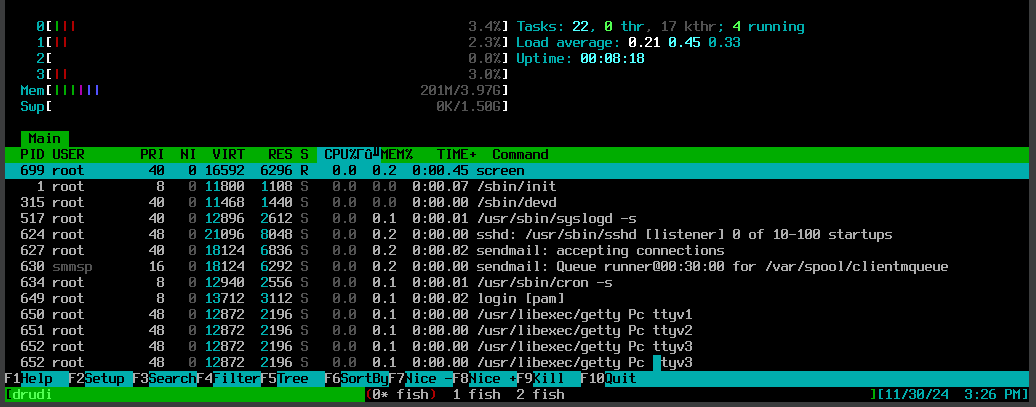
\includegraphics[width=0.8\textwidth]{images/cpuOnOff-result-idle.png}
    \caption{Estado inactivo del sistema.}
    \label{fig:cpuOnOff-result-idle}
\end{figure}

\subsection{Comportamiento con el Módulo Inhabilitado}
Cuando el módulo de encendido/apagado de procesadores no está habilitado para ningún núcleo, el sistema operativo sigue su funcionamiento convencional bajo la lógica del planificador. En este estado, el \textit{scheduler} opera mediante el uso de la Red de Petri  con las plazas y transiciones de cada uno de los procesadores del sistema, sin hacer uso de la adición de plazas y transiciones que corresponden al módulo, introducidas en el desarrollo del mismo.\par

Para confirmar dicho comportamiento, llevamos a cabo una prueba de estrés sobre los procesadores, ejecutando un programa que genera múltiples procesos que realizan cálculos matemáticos complejos. Durante la ejecución del programa, supervisamos el sistema y observamos que todos los procesadores operaban al máximo de su capacidad, funcionando al 100\% para completar la tarea. La Figura \ref{fig:cpuOnOff-result-full-load} proporciona una representación visual de este estado.\par

Este escenario de funcionamiento con el módulo deshabilitado proporciona un punto de referencia inicial para comprender el impacto de nuestra implementación en la gestión de recursos y el rendimiento general del sistema operativo.\par

\begin{figure}[H]
    \centering
    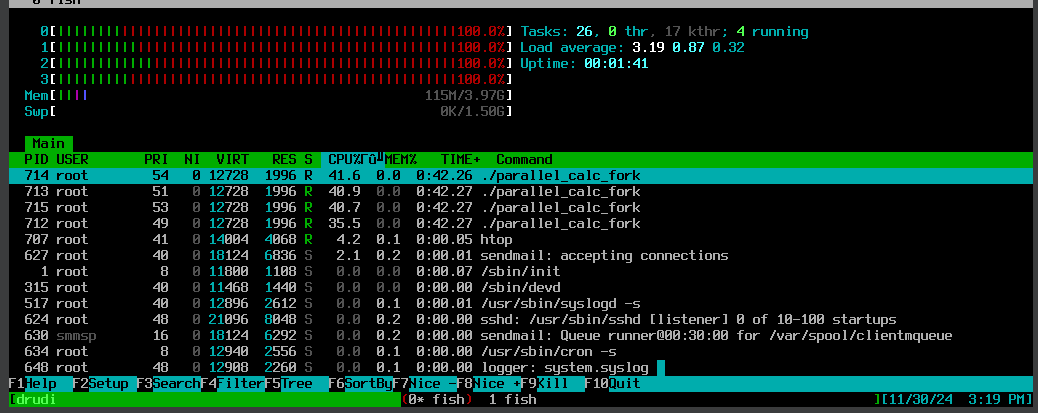
\includegraphics[width=0.8\textwidth]{images/cpuOnOff-result-full-load.png}
    \caption{Estado de los núcleos con el módulo encendido/apagado inhabilitado.}
    \label{fig:cpuOnOff-result-full-load}
\end{figure}

\subsection{Comportamiento con el Módulo Habilitado}
Basándonos en las observaciones anteriores, llevamos a cabo la misma prueba de estrés, pero activando previamente el módulo de encendido/apagado para inhabilitar el CPU2.\par

Este enfoque nos permitió no solo corroborar la funcionalidad adecuada de la implementación, sino también analizar la respuesta del sistema ante un cambio tan significativo como el bloqueo del encolado en uno de sus núcleos.\par

En relación a los resultados obtenidos durante esta evaluación, observamos que, al suspender uno de los procesadores del sistema, este continuó funcionando de manera estable. Se puede apreciar que la carga del procesador suspendido se mantuvo en cero, mientras que los demás procesadores continuaron ejecutando los cálculos. Esto demuestra de manera concluyente que el sistema fue capaz de adaptarse sin dificultades a la reducción de recursos de procesamiento.\par

\begin{figure}[H]
    \centering
    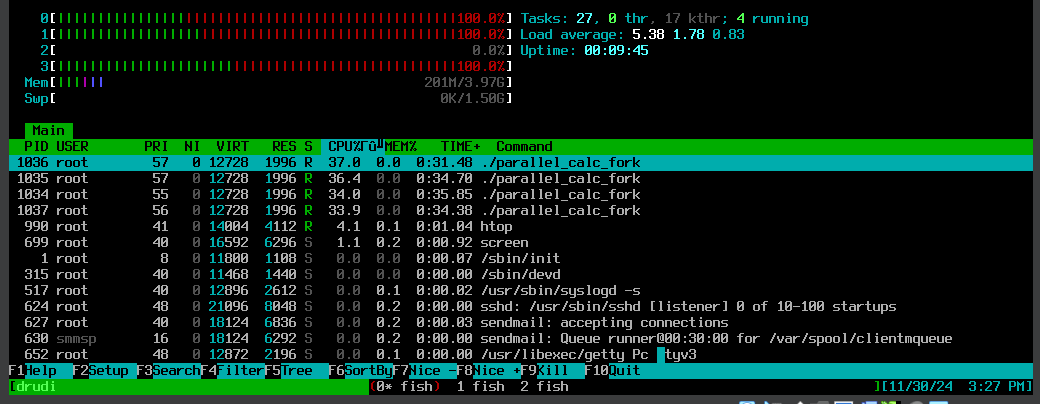
\includegraphics[width=0.8\textwidth]{images/cpuOnOff-result-1CPU.png}
    \caption{Estado de los núcleos con el módulo encendido/apagado habilitado para la CPU2.}
    \label{fig:cpuOnOff-result-1cpu}
\end{figure}

En relación al tiempo necesario para completar el cálculo del programa, notamos que dicho tiempo aumentó proporcionalmente a la disminución en el número de procesadores activos, destacando la correlación entre la disponibilidad de recursos de procesamiento y el tiempo total requerido para finalizar el programa. En la Figura \ref{fig:cpuOnOff-result-2cpu} podemos comprobar el funcionamiento del sistema con la inhabilitación simultánea de dos procesadores.\par

\begin{figure}[H]
    \centering
    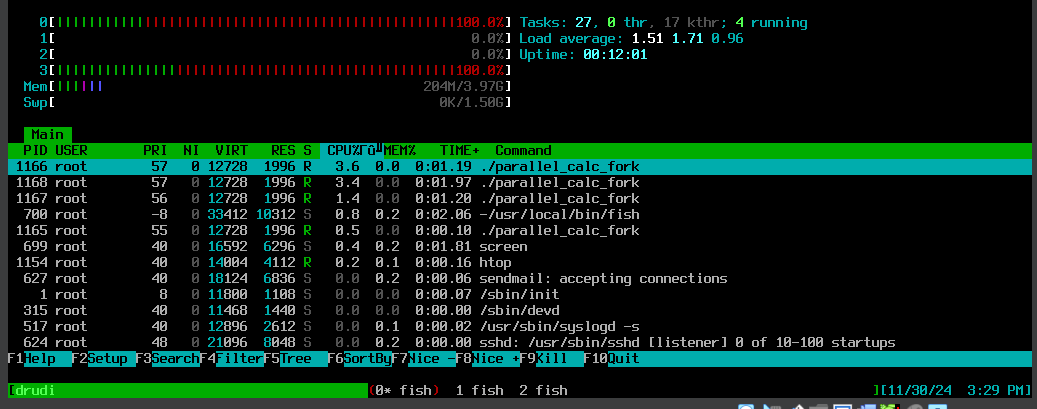
\includegraphics[width=0.8\textwidth]{images/cpuOnOff-result-2CPU.png}
    \caption{Estado de los núcleos con el módulo encendido/apagado habilitado para múltiples CPUs.}
    \label{fig:cpuOnOff-result-2cpu}
\end{figure}

En la Tabla \ref{tabla:cpuOnOff-result-times} se presentan los tiempos de ejecución del programa de estrés con diferentes cantidades de CPUs activos. Estos resultados confirman la relación entre la cantidad de procesadores activos y el tiempo necesario para completar la tarea.\par

\begin{table}[H]
    \centering
    \begin{tabular}{|c|c|c|c|c|}
        \hline
        \textbf{Cantidad de núcleos} & \textbf{4 CPUs} & \textbf{3 CPUs} & \textbf{2 CPUs} \\
        \hline
        \textbf{Tiempo} (segundos)   & 26              & 34              & 49              \\
        \hline
    \end{tabular}
    \caption{Tiempo de ejecución del programa de estrés con diferentes cantidades de CPUs activos.}
    \label{tabla:cpuOnOff-result-times}
\end{table}

El objetivo de esta prueba no es fomentar la suspensión de procesadores durante un contexto de gran carga de trabajo, sino demostrar la capacidad del sistema para adaptarse a la reducción de recursos de procesamiento. En el futuro, se espera que el \textit{kernel} sea quien decida de forma autónoma, cuándo suspender procesadores para lograr una mayor eficiencia energética.\par

Las capturas de pantalla con los resultados mostrados en la Tabla \ref{tabla:cpuOnOff-result-times} se encuentran documentados en el Apéndice \ref{appendix:apD}.


\section{Resultados del Módulo de Monopolización de Núcleos}

El módulo de monopolización de núcleos cumple su objetivo, permitiendo que un hilo se ejecute exclusivamente en un procesador sin que otros hilos sean encolados en él. Para validar su funcionamiento, realizamos la siguiente prueba:

\begin{enumerate}
    \item \textbf{Estado normal del sistema:} Con el módulo deshabilitado, los hilos se distribuyen entre los procesadores disponibles según las políticas de planificación definidas por la Red de Petri.
    \item \textbf{Comportamiento con el módulo habilitado:} Se seleccionó un hilo y se lo ancló a un procesador específico. Como resultado, el hilo permaneció en ejecución en el mismo núcleo durante toda la prueba, sin migraciones a otros procesadores ni interferencias de otros hilos.
\end{enumerate}

Estos resultados confirman que el sistema es capaz de asignar núcleos exclusivos a hilos específicos sin afectar la estabilidad general del planificador.\par

En los siguientes apartados se detallan las observaciones y análisis específicos de cada etapa de la prueba.\par

\subsection{Estado Normal del Sistema}

En este apartado se analizará el comportamiento general del sistema con el módulo de monopolización deshabilitado. Es relevante señalar que bajo esta configuración, los procesadores operan de forma predeterminada, utilizando la Red de Petri como planificador para mantener el equilibrio de la carga. De esta forma, los núcleos que en algún momento carezcan de tareas tomarán hilos de la cola global o ejecutaran hilos de clase IDLE en caso de inactividad del sistema. Con el planificador funcionando normalmente, los subprocesos se distribuyen entre los núcleos disponibles, utilizando las políticas definidas por el mismo.\par

En la Figura \ref{fig:top_disabled} se puede observar el estado de los procesos en el sistema con el módulo de monopolización deshabilitado. En este caso, se puede apreciar que los procesos se distribuyen de manera equitativa entre los núcleos, sin que ninguno de ellos monopolice un núcleo específico.\par

A su vez se ha ejecutado el proceso de estrés configurado para tener un solo hilo de procesamiento y así poder observar como el sistema opera en condiciones normales, reorganizando los tiempos de cada procesador para equilibrar la carga.\par

\begin{figure}[H]
    \centering
    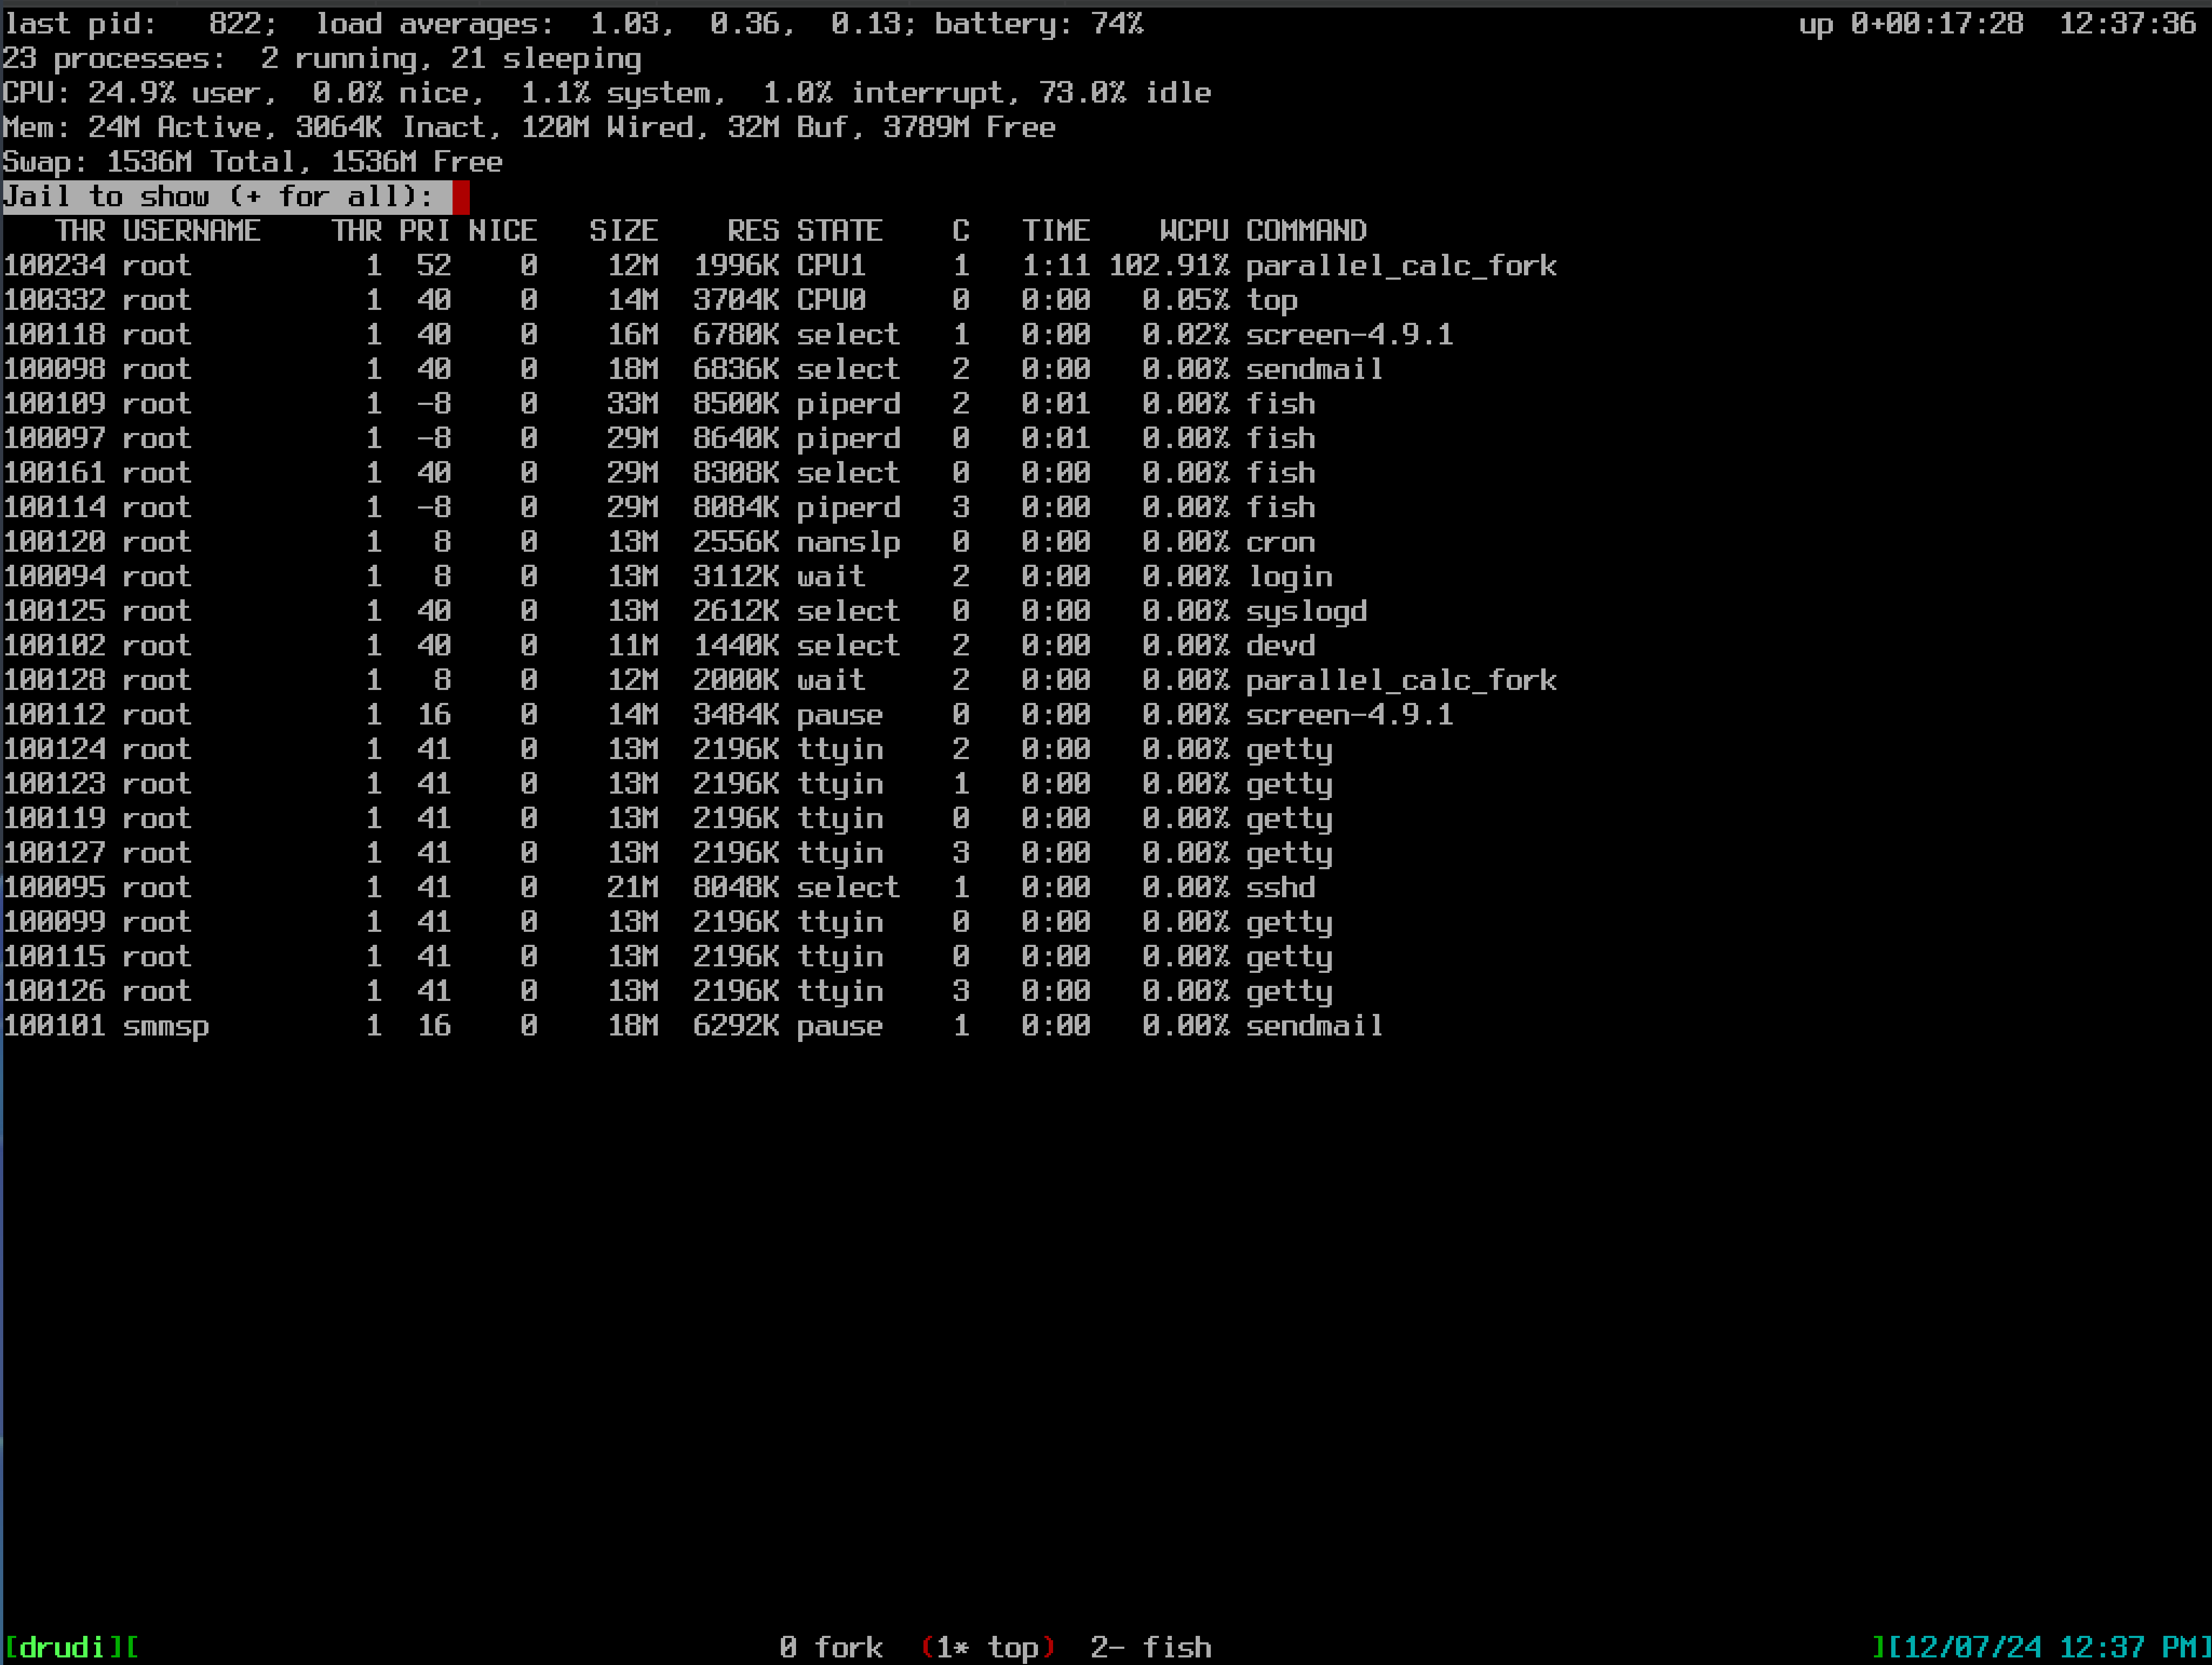
\includegraphics[width=1\textwidth]{images/top_disabled.png}
    \caption{Estado de los procesos en el sistema con el módulo de monopolización deshabilitado.}
    \label{fig:top_disabled}
\end{figure}

Además de los resultados obtenidos con la herramienta que monitora los procesos del sistema, se ha ejecutado otro programa encargado de hacer un seguimiento a un hilo determinado, mostrando los cambios de procesador en tiempo real. En la Figura \ref{fig:dtrace_disabled} se puede observar el comportamiento del hilo con el módulo de monopolización deshabilitado, donde se aprecia como este se ejecuta en diferentes núcleos del sistema.\par

\begin{figure}[H]
    \centering
    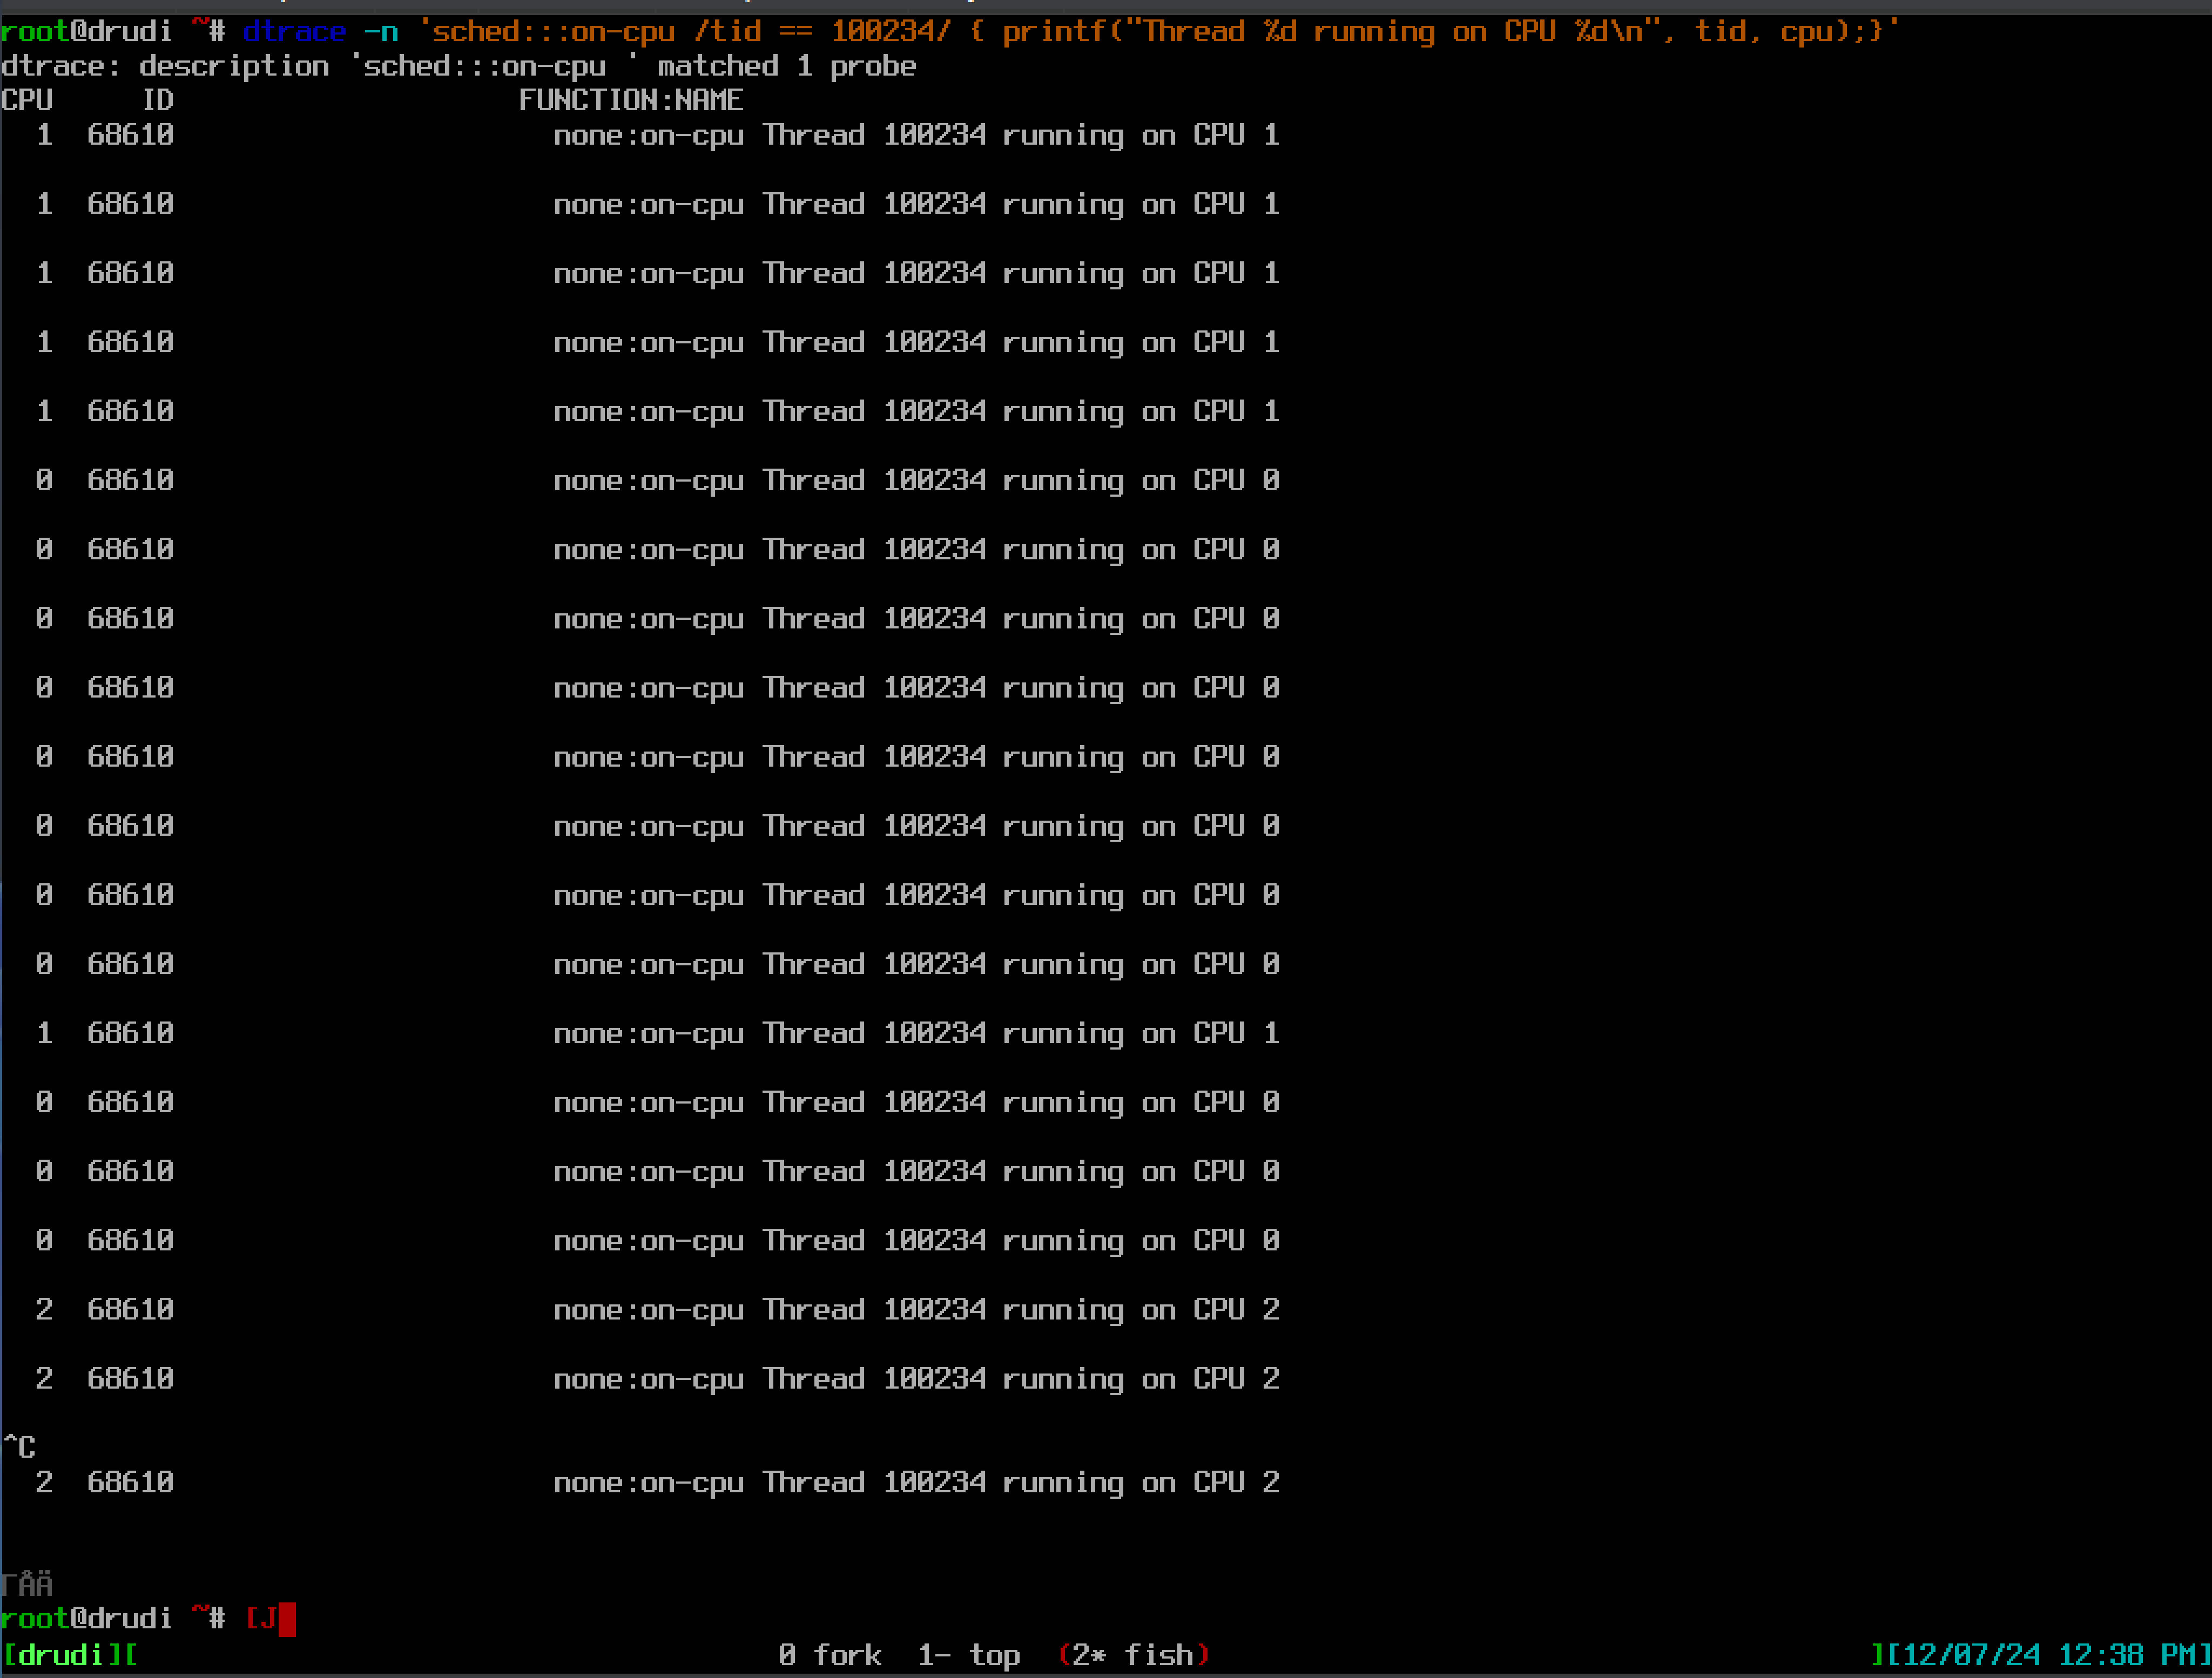
\includegraphics[width=1\textwidth]{images/dtrace_disabled.png}
    \caption{Ejecución de un hilo en diferentes núcleos del sistema con el módulo de monopolización deshabilitado.}
    \label{fig:dtrace_disabled}
\end{figure}


\subsection{Comportamiento con el Módulo Habilitado}
Habiendo expuesto el comportamiento del sistema en su condición normal, se sienta una base para la posterior comparación con el desempeño del módulo.\par

Siguiendo un procedimiento similar al empleado con el módulo de encendido y apagado, procedimos a ejecutar nuevamente el programa de estrés, orientado al cálculo de números primos.\par

Luego de haber activado el módulo podemos observar que los resultados obtenidos concuerdan con la información proporcionada por la  herramienta de monitoreo. Como era de esperar, este subproceso estuvo vinculado al CPU elegido, durante toda su ejecución. Además, ningún otro hilo o proceso se ejecutó en ningún momento en este núcleo, evidenciando así su exclusividad y el correcto funcionamiento del desarrollo.\par

\begin{figure}[H]
    \centering
    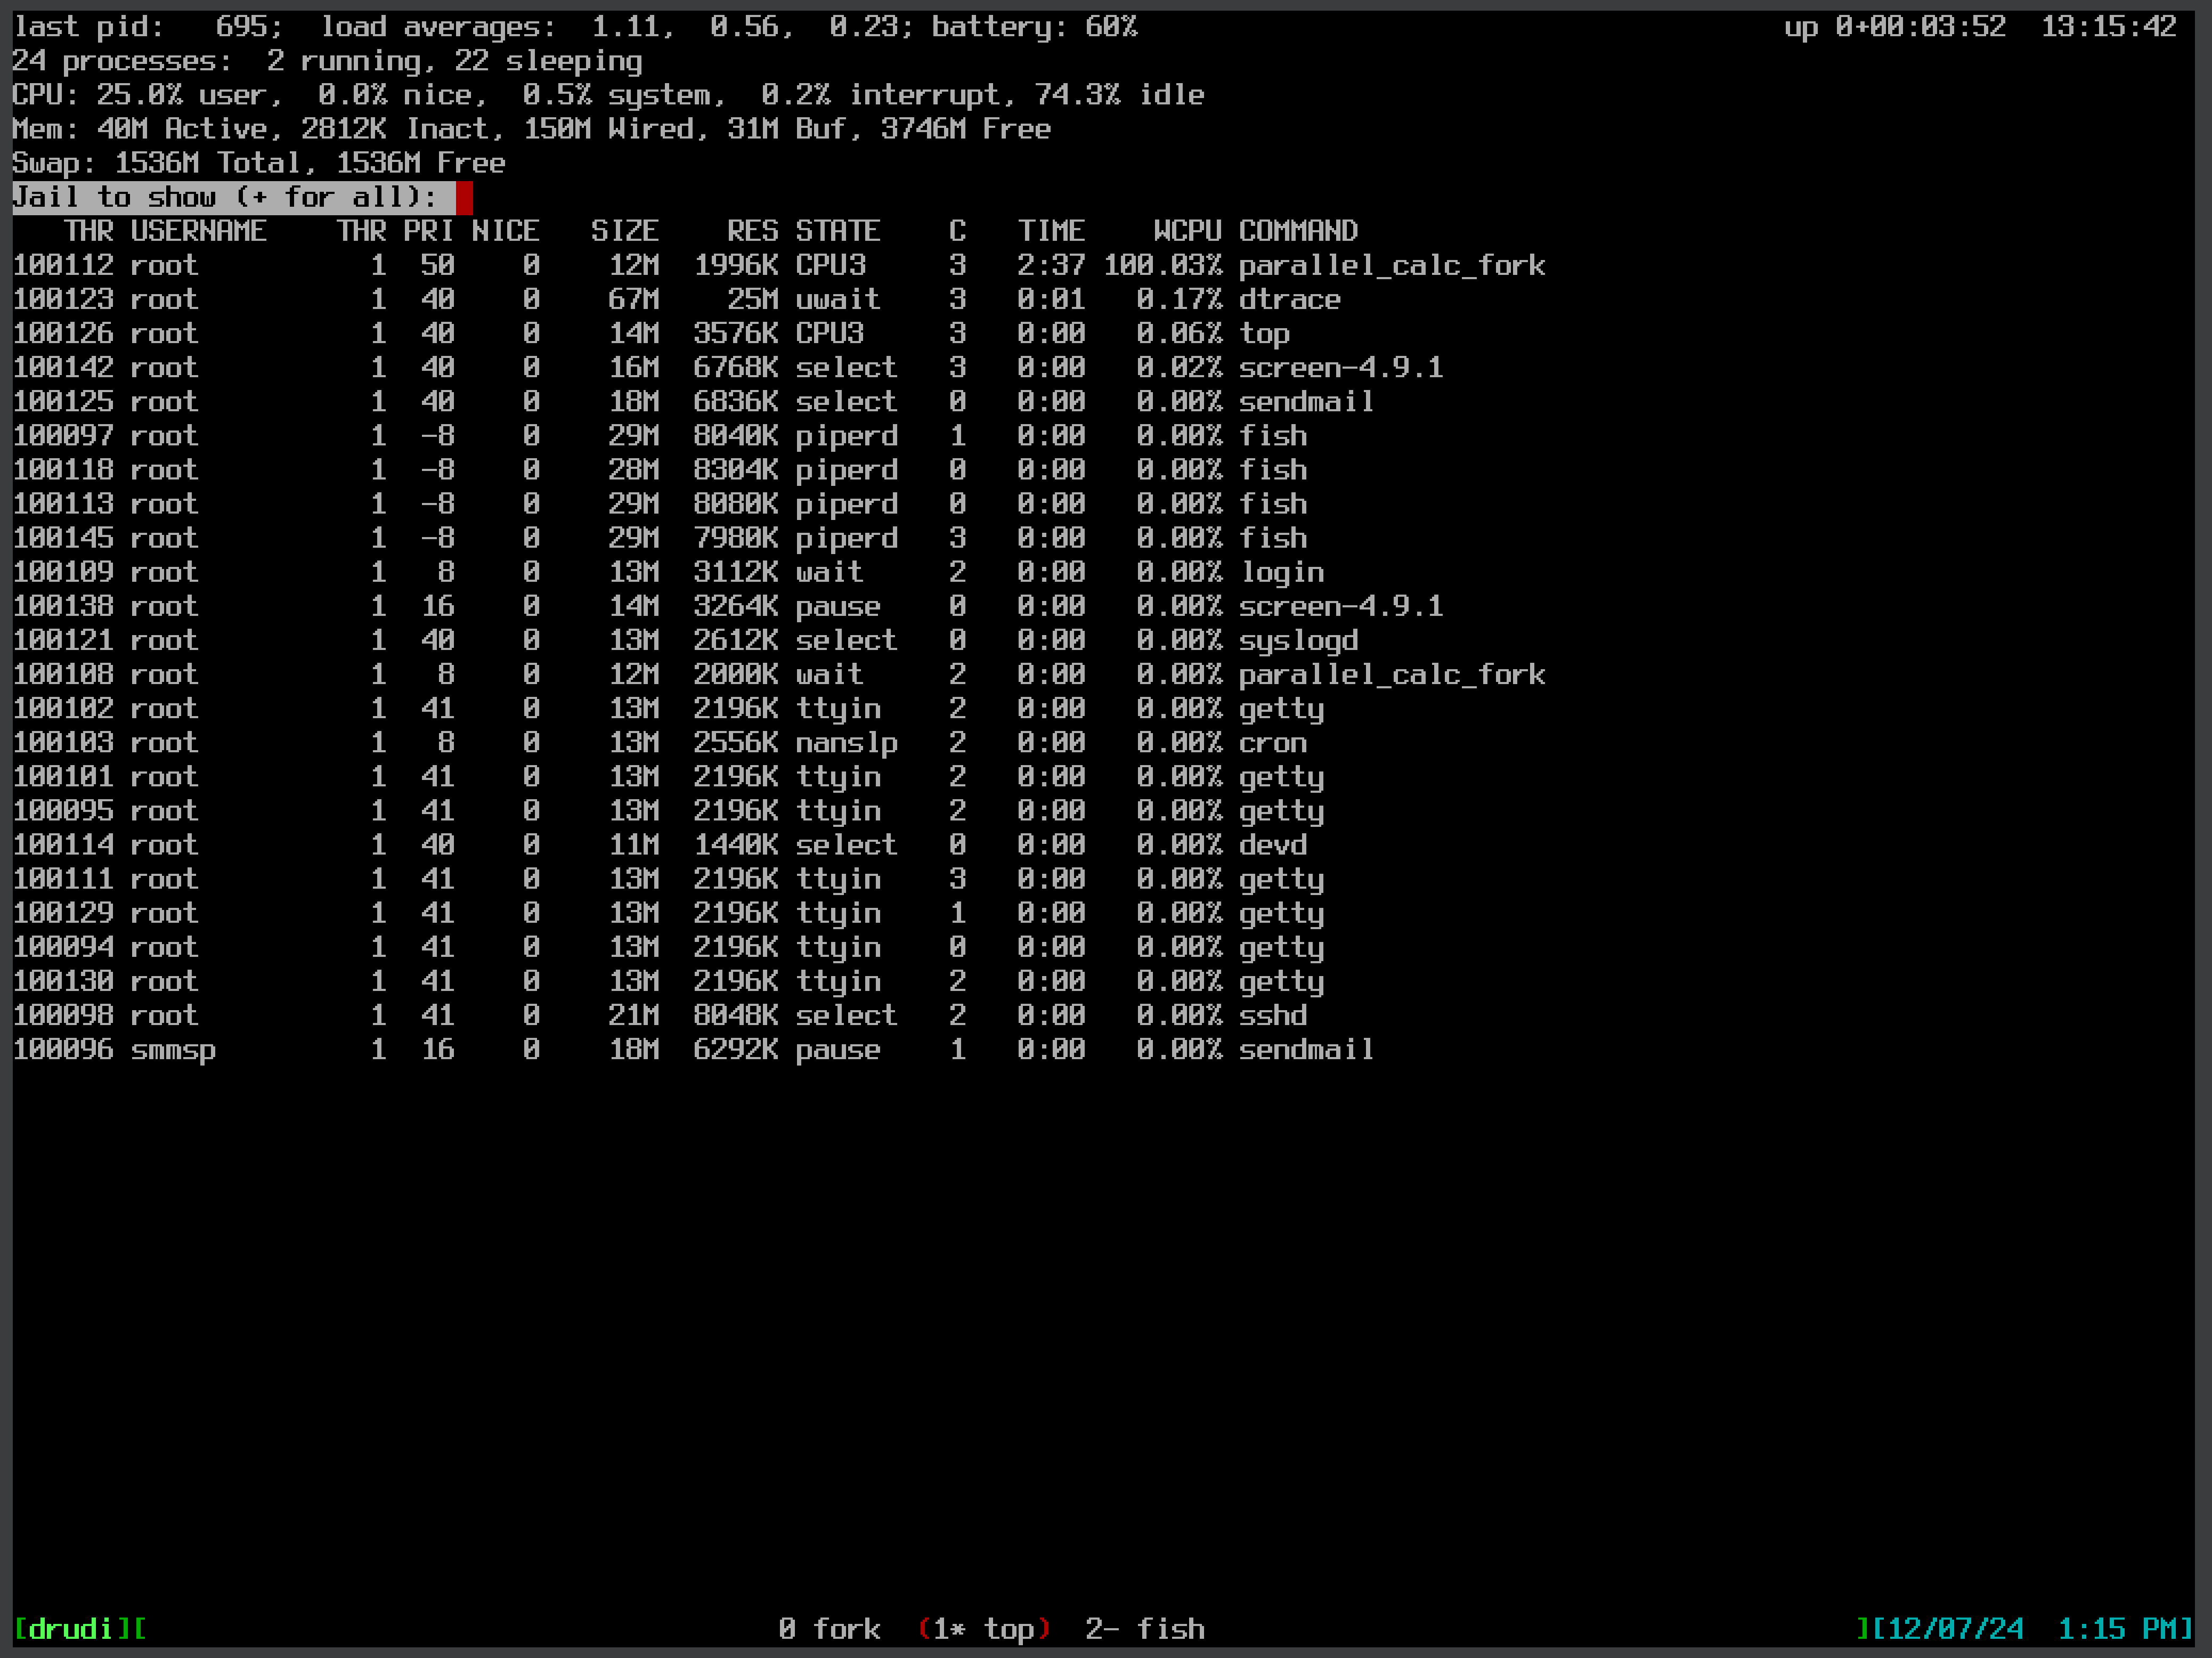
\includegraphics[width=1\textwidth]{images/cpuMonopolized-idle.png}
    \caption{Estado de los procesos previo a la habilitación del módulo.}
    \label{fig:cpuMonopolized-idle}
\end{figure}

\begin{figure}[H]
    \centering
    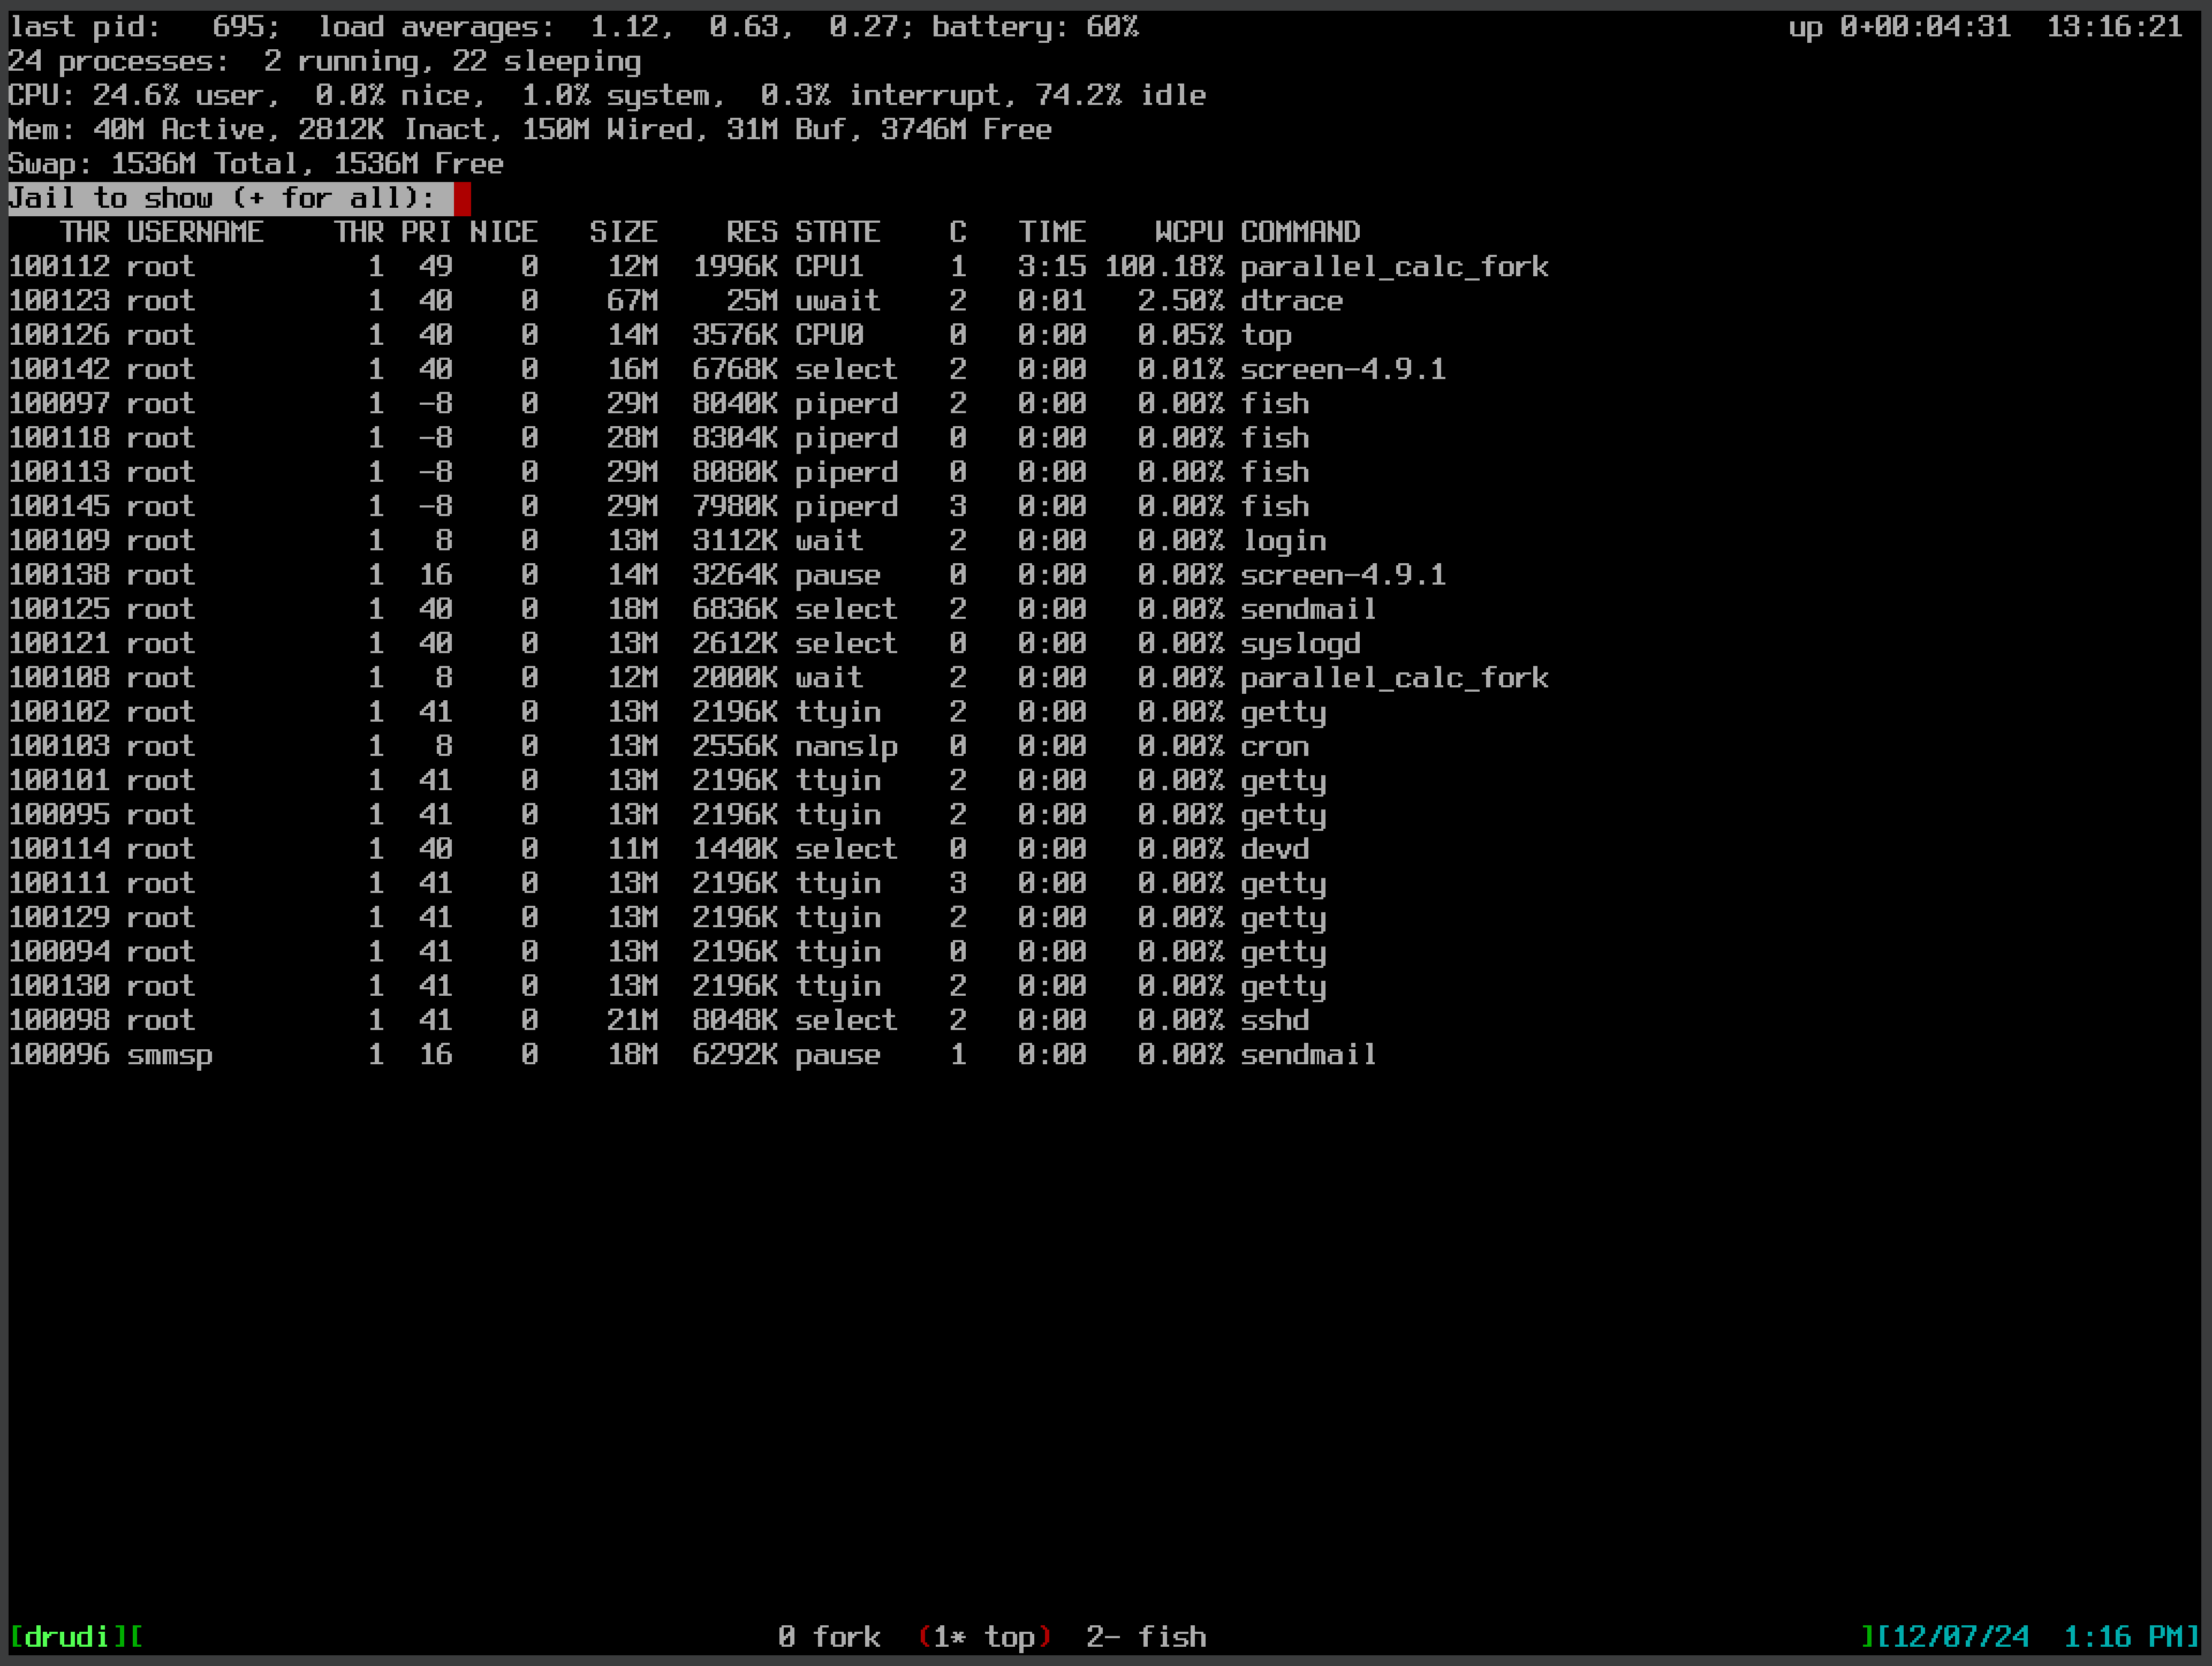
\includegraphics[width=1\textwidth]{images/cpuMonopolized-on.png}
    \caption{Estado de los procesos luego de activar el módulo de monopolización para el CPU1.}
    \label{fig:cpuMonopolized-on}
\end{figure}

En la Figura \ref{fig:cpuMonopolized-dtrace} se observa el comportamiento del hilo con respecto a los núcleos en los que se ejecuta, comenzando con una asignación de acuerdo al planificador y luego de la activación del módulo, se puede observar como el hilo se ejecuta en el núcleo designado.\par

\begin{figure}[H]
    \centering
    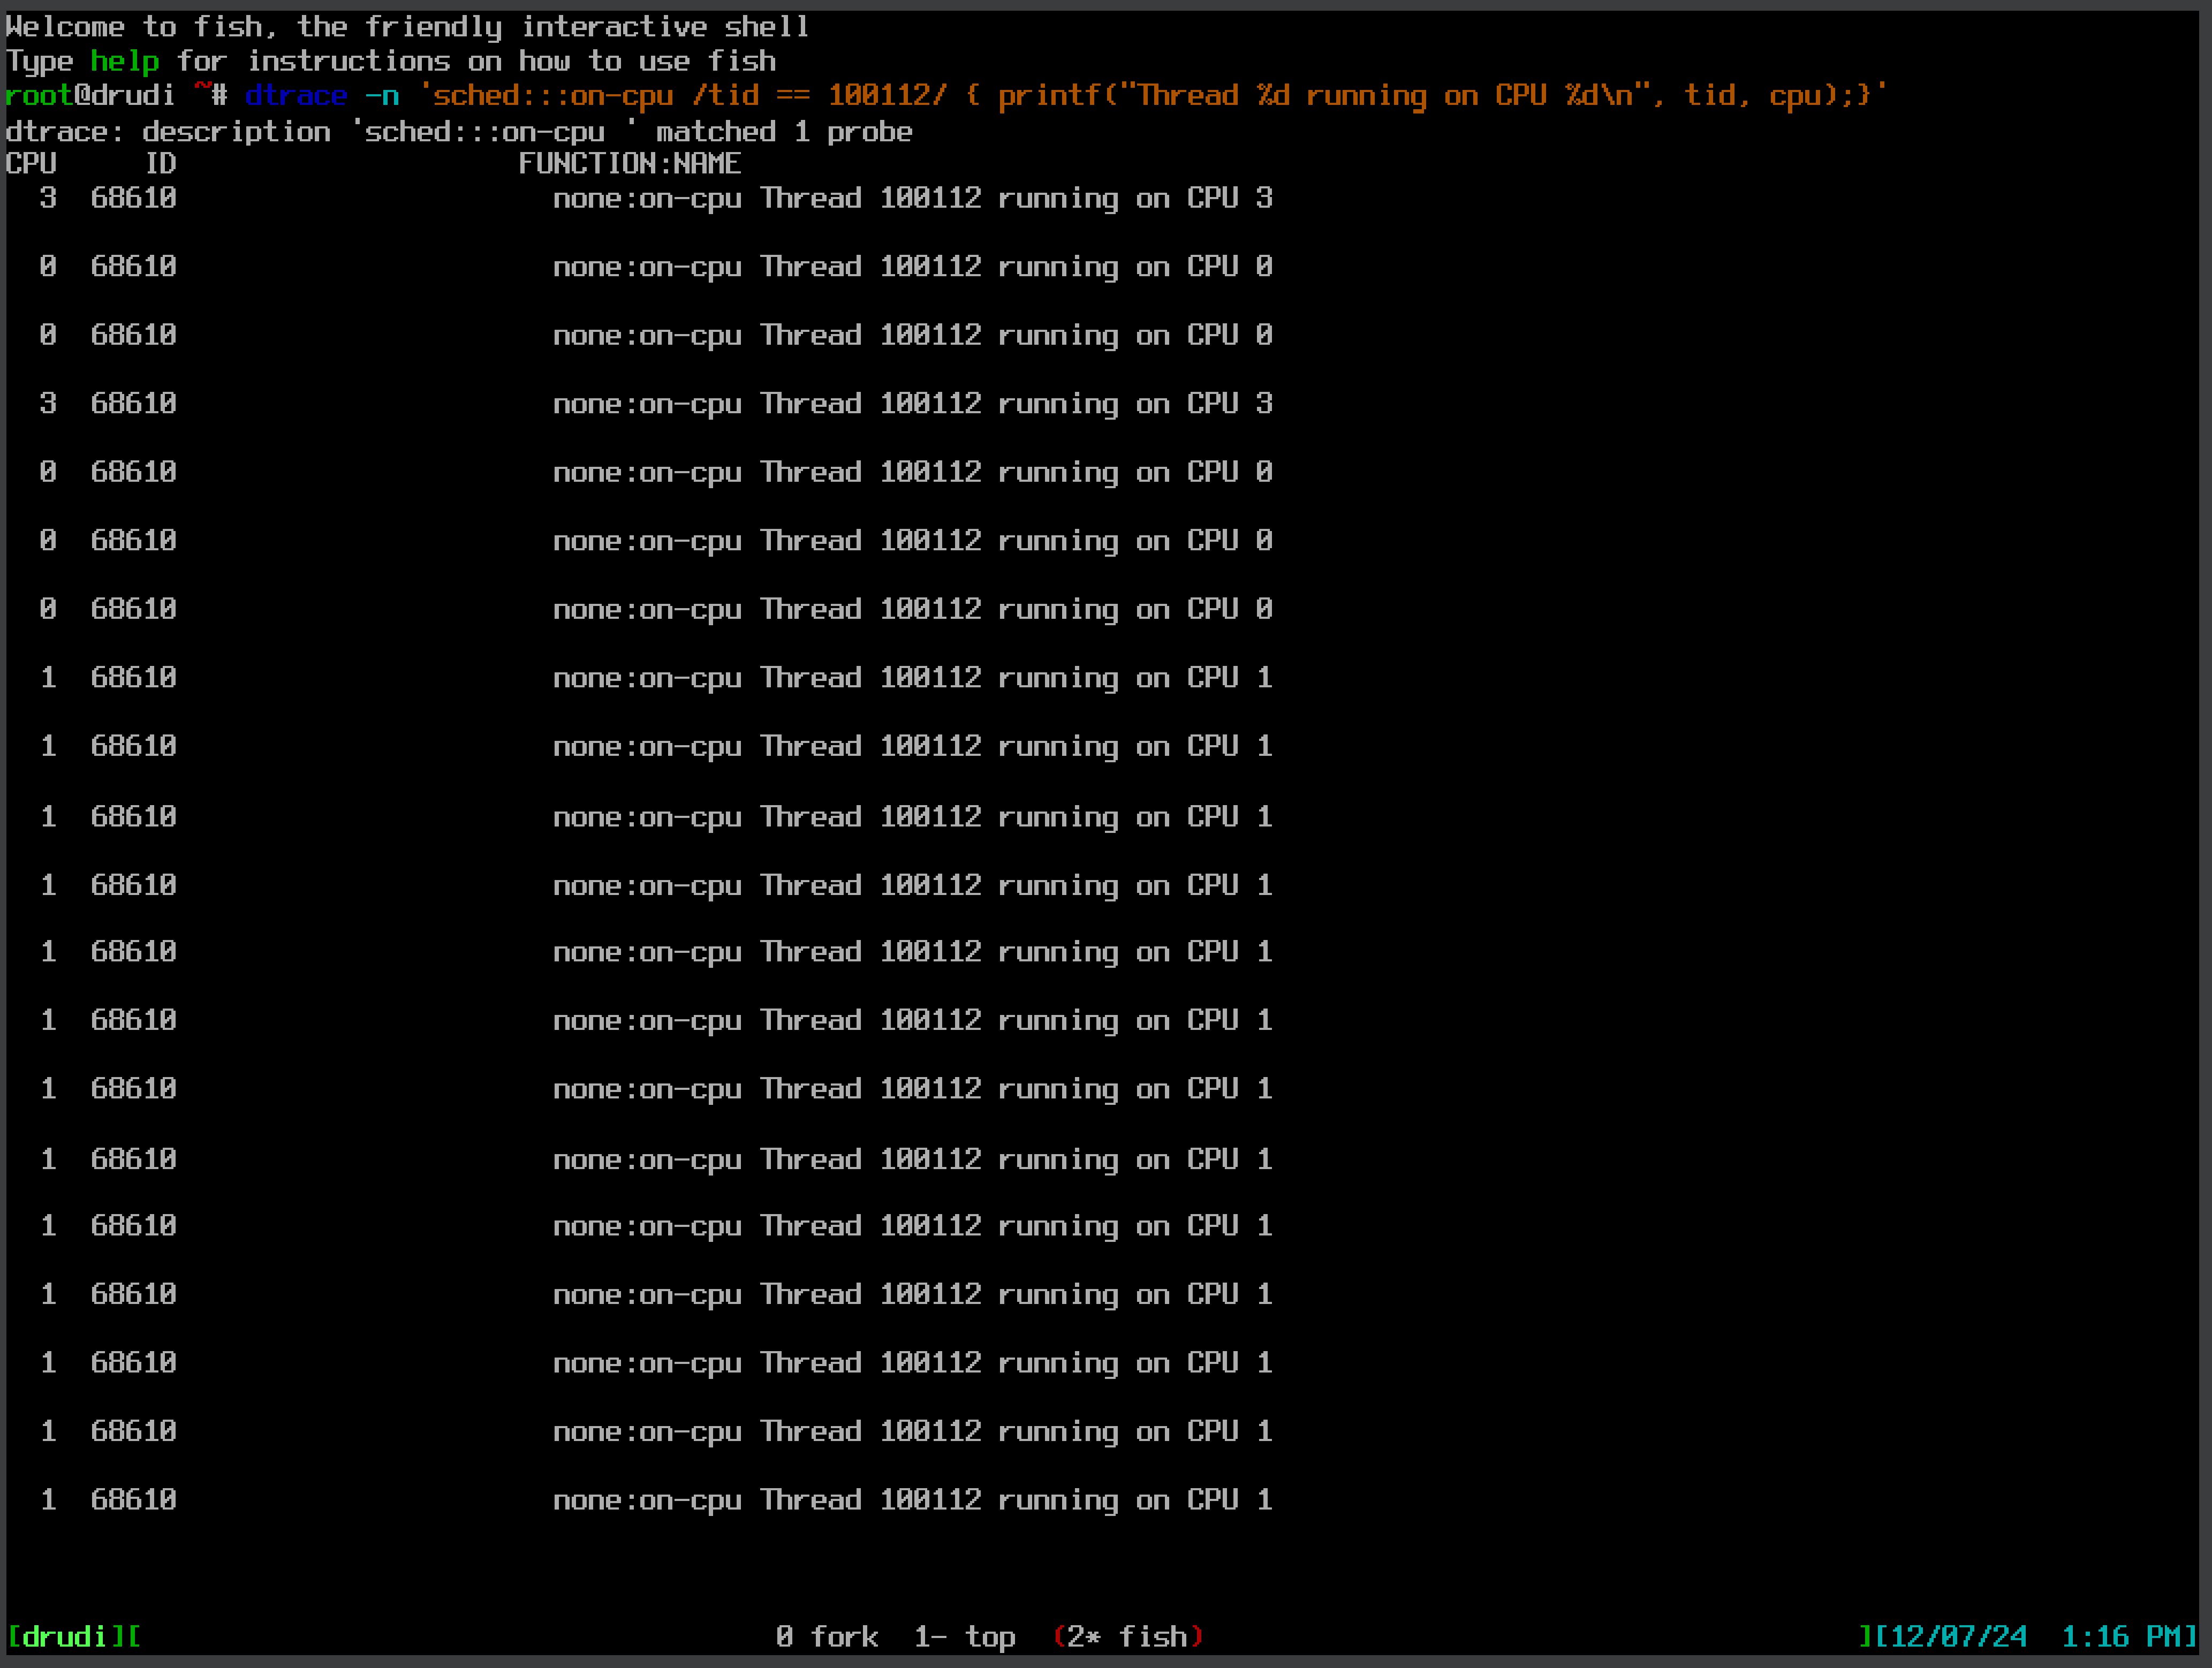
\includegraphics[width=1\textwidth]{images/cpuMonopolized-dtrace.png}
    \caption{Estado del hilo monopolizado antes y después de la activación del módulo.}
    \label{fig:cpuMonopolized-dtrace}
\end{figure}

Un caso relevante es el estado del sistema una vez que el programa de estrés ha concluido pero el módulo permanece activado. En estas condiciones, se observa cómo el núcleo al que se había anclado el hilo permanece “reservado”, sin ejecutar ningún hilo que no posea el identificador especificado, mientras que los procesos restantes solo se ejecutan en los núcleos liberados. Con esto en mente, se puede identificar una similitud con el funcionamiento del módulo de encendido/apagado al desactivar un núcleo.\par

Al desactivar el módulo, el sistema continúa operando según lo esperado, con todos sus núcleos disponibles, tal como lo haría en su estado normal.\par

\section{Resultados de las actualizaciones en la versión del S.O.}

En esta sección se presentan los resultados de las actualizaciones realizadas para adaptar el planificador basado en Redes de Petri a las versiones más recientes del sistema operativo, particularmente la versión 13.1. Estas actualizaciones aseguraron la continuidad del rendimiento observado originalmente en la versión 11, sincronizando el proyecto con la última versión estable del sistema.\par

La actualización fue priorizada al inicio del proyecto para mantenernos alineados con la comunidad y facilitar el desarrollo sobre una base de código actualizada. Esto permitió reducir las diferencias entre el \textit{kernel} original y nuestro \textit{fork}, optimizando su integración en etapas posteriores. Si bien fue necesario resolver diversos conflictos entre las versiones 11 y 13 de FreeBSD, las pruebas confirmaron que el planificador opera de manera estable en la versión actualizada.\par

El código actualizado se encuentra en una rama específica del repositorio, junto con ramas adicionales que documentan cada etapa de la transición progresiva desde la versión 11 hasta la 13.1.\par

